\documentclass[11pt,a4paper]{article}

\usepackage[margin=2.2cm]{geometry}
\usepackage{graphicx}
\usepackage{booktabs}
\usepackage{tabularx}
\usepackage{array}
\usepackage{caption}
\usepackage{float}
\usepackage{xcolor}
\usepackage{tikz}
\usepackage[hidelinks]{hyperref}
\usetikzlibrary{arrows.meta, positioning, shapes.geometric}

\graphicspath{{../../part1/assets/brand/}{../}}

\definecolor{accent}{HTML}{0E6B67}
\definecolor{softgray}{HTML}{F4F6F6}
\definecolor{midgray}{HTML}{666666}
\definecolor{softaccent}{HTML}{E7F4F2}
\definecolor{softgold}{HTML}{FFF4D6}

\setlength{\parindent}{0pt}
\setlength{\parskip}{0.6em}
\renewcommand{\arraystretch}{1.15}
\captionsetup{labelsep=period}
\newcolumntype{L}[1]{>{\raggedright\arraybackslash}p{#1}}
\newcolumntype{Y}{>{\raggedright\arraybackslash}X}

\newcommand{\placeholder}[1]{%
    \textcolor{midgray}{\textit{[#1]}}%
}

\newcommand{\frameworknote}[2]{%
    \begin{center}
        \fcolorbox{accent}{softaccent}{%
            \begin{minipage}{0.92\textwidth}
                \textbf{#1}\\[0.35em]
                \small #2
            \end{minipage}%
        }
    \end{center}
}

\newcommand{\placeholderfigure}[3]{%
    \begin{figure}[H]
        \centering
        \fcolorbox{midgray}{softgray}{%
            \begin{minipage}[c][#2][c]{0.9\textwidth}
                \centering
                \textbf{#1}\\[0.5em]
                \small \placeholder{Insert the final artefact here.}
            \end{minipage}%
        }
        \caption{#1.}
        \label{#3}
    \end{figure}
}

\begin{document}
\pagenumbering{gobble}

\begin{titlepage}
    \centering
    \vspace*{0.2cm}
    
\includegraphics[width=4.2cm]{unsw_logo.png}

    \vspace{1.1cm}
    {\Large DESN2000 SENG\par}
    \vspace{0.3cm}
    {\Huge\bfseries Part 2 Group Report\par}
    \vspace{0.25cm}
    {\Large LaTeX Framework\par}

    \vspace{1.2cm}
    \begin{tabularx}{0.88\textwidth}{@{}L{3.2cm}Y@{}}
        Project title & \placeholder{Insert project title}\\
        Team members & \placeholder{Insert team member names and zIDs}\\
        Submission date & \placeholder{Insert submission date}\\
    \end{tabularx}

    \vfill
\end{titlepage}

\pagenumbering{roman}
\tableofcontents
\newpage
\pagenumbering{arabic}

\section{Introduction and Part 2 Scope}

Part~1 used surveys and interviews with four stakeholder groups to define the problem and develop personas. This report applies the Ideate stage to that evidence. It compares three technical concepts, selects one through a weighted decision matrix, and translates the selected direction into a Jira backlog and a preliminary prototype.

The report focuses on the student journey from accommodation search to an agreed shared living arrangement. Property manager stories remain in the backlog as secondary scope.

\section{Problem Statement and Research Justification}

\subsection{Problem Statement}

The following statement was approved in Part~1 and is reproduced without alteration.

\begin{center}
    \fcolorbox{accent}{softaccent}{%
        \begin{minipage}{0.92\textwidth}
            \textit{Create a mobile platform which allows university students and shared accommodation residents to seamlessly manage household responsibilities, expenses and housemate communication, while also enabling property managers to streamline tenancy administration and tenant communication, to reduce conflict between tenants, streamline property management, and improve the overall shared living experience.}
        \end{minipage}%
    }
\end{center}

The statement covers student and property manager needs. This report narrows the preliminary prototype to the student path. A student searches for an option, checks verification, compares compatibility, starts contact in the app, and acknowledges a household rule. Property manager functions remain outside Sprint~1.

\subsection{Research Justification}

Table~\ref{tabresearchtraceability} links the strongest Part~1 evidence to a user need and a backlog response. This traceability keeps the proposed features grounded in the research.

\begin{table}[H]
    \centering
    \small
    \caption{Research traceability.}
    \begin{tabularx}{\textwidth}{@{}Y Y Y@{}}
        \toprule
        Research evidence & User need & Backlog response\\
        \midrule
        All 16 international respondents reported concern about rental scams. A further 43.75\% had encountered misleading or false listing information. & The international student persona needs clear evidence about a profile or listing before making contact. & Show profile verification status in US-11 and clear listing details in US-13.\\
        87.5\% rated housemate compatibility as very or extremely important. A further 68.75\% had experienced conflict with a previous housemate. & The long term housemate persona needs to identify practical mismatches before committing. & Compare living preferences in US-12.\\
        44\% identified communication difficulty as the hardest part of the search. More than 80\% were willing to use preference based matching. & The international student persona needs first contact without early disclosure of personal details. & Keep first contact inside the app through US-09.\\
        All surveyed domestic students relied on verbal household agreements and had experienced conflict over responsibilities. A further 66.67\% wanted better chore tracking. & A new share house resident needs accepted expectations to remain visible after move in. & Store acknowledged household rules through US-02 and US-10.\\
        \bottomrule
    \end{tabularx}
    \label{tabresearchtraceability}
\end{table}

\section{Solution Ideation}

\subsection{Research to Ideation Transition}
\label{subsectransition}

The evidence in Table~\ref{tabresearchtraceability} was reframed as four design needs. Table~\ref{tabdesignneeds} sets the boundary for concept generation and later evaluation.

\begin{table}[H]
    \centering
    \small
    \caption{Research issues and design needs.}
    \begin{tabularx}{\textwidth}{@{}L{5.2cm}Y@{}}
        \toprule
        Research issue & Design need\\
        \midrule
        Scam concern and misleading information & Visible verification status and clear listing data\\
        Conflict caused by poor living fit & Structured preference comparison\\
        Risk during first contact & In app messaging before contact disclosure\\
        Verbal household expectations & Recorded rules with acknowledgement\\
        \bottomrule
    \end{tabularx}
    \label{tabdesignneeds}
\end{table}

The resulting design question was as follows.

\begin{center}
    \fcolorbox{accent}{softaccent}{%
        \begin{minipage}{0.92\textwidth}
            \centering
            \textit{How might we help students move from an uncertain accommodation search to an informed shared living agreement?}
        \end{minipage}%
    }
\end{center}

Each concept was assessed against this question.

\subsection{Generated Technical Concepts}
\label{subsecgeneratedconcepts}

The team generated three concepts with different technical boundaries. Table~\ref{tabconceptoverview} gives the comparison. Tables~\ref{tabconcepta} to \ref{tabconceptc} describe how each concept operates.

\begin{table}[H]
    \centering
    \small
    \caption{Overview of the generated concepts.}
    \begin{tabularx}{\textwidth}{@{}L{1.4cm}L{4.1cm}Y Y@{}}
        \toprule
        Concept & Name & Main user task & Technical boundary\\
        \midrule
        A & Verified Contact Gateway & Check status before first contact & Verification state and protected messaging\\
        B & Explainable Compatibility Matcher & Compare practical living fit & Preference model and explainable score\\
        C & Trust to Agreement Journey & Move from search to an acknowledged rule & Integrated flow across the core services\\
        \bottomrule
    \end{tabularx}
    \label{tabconceptoverview}
\end{table}

\begin{table}[H]
    \centering
    \small
    \caption{Concept A. Verified Contact Gateway.}
    \begin{tabularx}{\textwidth}{@{}L{3.2cm}Y@{}}
        \toprule
        Aspect & Description\\
        \midrule
        Purpose & Reduce uncertainty during first contact with an unfamiliar person.\\
        Operation & The system records each verification check as \textit{unverified}, \textit{pending}, \textit{verified}, \textit{rejected} or \textit{expired}. The interface shows the status and hides submitted evidence. Messaging does not expose personal contact details.\\
        Research fit & Responds to scam concern and reluctance to contact unknown people.\\
        Limitation & A verified identity does not establish compatibility or future conduct.\\
        \bottomrule
    \end{tabularx}
    \label{tabconcepta}
\end{table}

\begin{table}[H]
    \centering
    \small
    \caption{Concept B. Explainable Compatibility Matcher.}
    \begin{tabularx}{\textwidth}{@{}L{3.2cm}Y@{}}
        \toprule
        Aspect & Description\\
        \midrule
        Purpose & Help users identify practical mismatches before committing.\\
        Operation & Users record living preferences and mark mandatory constraints. The matcher removes candidates who breach a mandatory constraint. It then calculates a weighted score and shows the factors that affected the result.\\
        Research fit & Responds to the importance of daily living compatibility in the Part~1 findings.\\
        Limitation & The score supports discussion but cannot predict a successful household.\\
        \bottomrule
    \end{tabularx}
    \label{tabconceptb}
\end{table}

\begin{table}[H]
    \centering
    \small
    \caption{Concept C. Trust to Agreement Journey.}
    \begin{tabularx}{\textwidth}{@{}L{3.2cm}Y@{}}
        \toprule
        Aspect & Description\\
        \midrule
        Purpose & Connect the accommodation decision with an explicit household agreement.\\
        Operation & The flow links profile setup, status display, compatibility comparison, in app contact, and rule acknowledgement. Each step passes only the data needed by the next step. Later household tools remain outside the first release.\\
        Research fit & Connects uncertainty before move in with unclear expectations after move in.\\
        Limitation & Its wider scope raises delivery and privacy risk.\\
        \bottomrule
    \end{tabularx}
    \label{tabconceptc}
\end{table}

Concepts A and B isolate one decision in the user journey. Concept C integrates those decisions and adds agreement. All three remained candidates for the weighted evaluation.

\subsection{Ideation Outcome}
\label{subsecideationoutcome}

The ideation stage produced three candidates with different value and delivery risk. No concept was selected at this stage. All three entered the weighted decision matrix in Section~\ref{secconceptselection}.

\subsection{Ideation Method}
\label{subsecideationmethod}

\frameworknote{Required content}{Name and explain the ideation method used by the team. Show how the method started from the problem definition and produced multiple ideas. Include evidence from the actual ideation activity.}

\begin{table}[H]
    \centering
    \small
    \caption{Ideation method template.}
    \begin{tabularx}{\textwidth}{@{}L{3.1cm}Y Y Y@{}}
        \toprule
        Ideation stage & Method used & Team activity & Output\\
        \midrule
        \placeholder{Stage 1} & \placeholder{Method} & \placeholder{What the team did} & \placeholder{Produced artefact}\\
        \placeholder{Stage 2} & \placeholder{Method} & \placeholder{What the team did} & \placeholder{Produced artefact}\\
        \placeholder{Stage 3} & \placeholder{Method} & \placeholder{What the team did} & \placeholder{Produced artefact}\\
        \bottomrule
    \end{tabularx}
    \label{tabideationmethod}
\end{table}

\placeholderfigure{Ideation process and evidence}{5.2cm}{figideationevidence}

\section{Concept Selection and Prioritisation}
\label{secconceptselection}

\subsection{Selection Method}
\label{subsecselectionmethod}

The weighted decision matrix selected the concept. MoSCoW prioritisation then set the delivery scope. This separation prevented a broad concept from being treated as a commitment to deliver every related feature.

Each concept was rated from 1 to 5. A rating of 1 indicated poor fit. A rating of 3 indicated partial fit with material limits. A rating of 5 indicated full fit under the stated prototype assumptions. The weighted total was calculated as

\[
S_j = \sum_i w_i r_{ij}
\]

where $w_i$ is the criterion weight and $r_{ij}$ is the rating for concept $j$.

\begin{table}[H]
    \centering
    \small
    \caption{Selection criteria and weights.}
    \begin{tabularx}{\textwidth}{@{}L{4.0cm}L{1.3cm}Y@{}}
        \toprule
        Criterion & Weight & Rationale\\
        \midrule
        Research evidence fit & 30\% & Measures direct traceability to the Part~1 findings and personas.\\
        User risk reduction & 20\% & Measures how much evidenced user risk the concept reduces.\\
        Feasibility within ten weeks & 20\% & Measures whether the team can prototype and revise the concept within the schedule.\\
        Prototype testability & 15\% & Measures whether users can complete observable tasks in a clickable flow.\\
        Innovation beyond isolated tools & 10\% & Measures whether the concept creates a research grounded journey rather than copying one existing function.\\
        Accessibility and privacy risk & 5\% & Measures whether foreseeable risks can be controlled. An unacceptable risk remains a rejection condition.\\
        \bottomrule
    \end{tabularx}
    \label{tabcriterionorigin}
\end{table}

The final ratings in Table~\ref{tabconceptselection} must match the scoring evidence in Figure~\ref{figselectionevidence}.

\placeholderfigure{Week 6 concept-selection evidence: independent ratings and consensus discussion}{4.5cm}{figselectionevidence}

\subsection{Decision Matrix}

The weighted total is the sum of each rating multiplied by its weight. The maximum score is 5.00.

\begin{table}[H]
    \centering
    \small
    \caption{Weighted decision matrix.}
    \begin{tabularx}{\textwidth}{@{}Y L{1.5cm}L{1.7cm}L{1.7cm}L{1.7cm}@{}}
        \toprule
        Selection criterion & Weight & Concept A & Concept B & Concept C\\
        \midrule
        Research evidence fit & 30\% & 4 & 4 & 5\\
        User risk reduction & 20\% & 4 & 4 & 5\\
        Feasibility within ten weeks & 20\% & 5 & 4 & 3\\
        Prototype testability & 15\% & 4 & 5 & 4\\
        Innovation beyond isolated tools & 10\% & 3 & 4 & 5\\
        Accessibility and privacy risk & 5\% & 4 & 4 & 3\\
        \midrule
        Weighted total & 100\% & \textbf{4.10} & \textbf{4.15} & \textbf{4.35}\\
        \bottomrule
    \end{tabularx}
    \label{tabconceptselection}
\end{table}

Concept C ranks first with 4.35. It fits the research and covers more of the target journey. Its lower feasibility and privacy rating exposes the main delivery risk.

\subsection{Selected Concept and Rationale}

Concept C was selected because it links the strongest research findings in one user path. Concept A stops after safer first contact. Concept B stops after the match decision. Concept C continues to an acknowledged household rule.

The preliminary prototype uses a narrow release slice to control scope. Table~\ref{tabmoscow} aligns the priority of every story with the Sprint~1 path shown later in the report.

% Confirm the non Sprint 1 allocations against the team Jira board before submission.
\begin{table}[H]
    \centering
    \small
    \caption{MoSCoW priorities for preliminary prototype delivery.}
    \begin{tabularx}{\textwidth}{@{}L{2.7cm}L{4.0cm}Y@{}}
        \toprule
        Priority & User stories & Delivery decision\\
        \midrule
        Must have in Sprint~1 & US-02, US-09, US-10, US-11, US-12, US-13 & These stories form one testable path from search to an acknowledged rule.\\
        Should have later & US-01, US-03, US-04, US-05, US-06, US-14 & These stories extend the agreement into routine household follow through.\\
        Could have & US-07, US-08, US-15 & These stories add supporting communication or reputation value without blocking the core path.\\
        Will not have in the preliminary prototype & US-16, US-17, US-18 & These stories introduce a separate role and additional permissions. They remain in the product backlog.\\
        \bottomrule
    \end{tabularx}
    \label{tabmoscow}
\end{table}

Only the Must have row defines Sprint~1. The same release slices are used in the backlog tables and must match Jira.

\section{Product Backlog Structure}
\label{secbacklog}

\subsection{Epic Overview}

The backlog contains four Epics. Each Epic groups stories that deliver a distinct user outcome. Stable story identifiers preserve links between this report, Jira, acceptance criteria, and prototype evidence.

\begin{table}[H]
    \centering
    \small
    \caption{Epic structure of the product backlog.}
    \begin{tabularx}{\textwidth}{@{}L{1.4cm}L{3.6cm}Y L{3.4cm}@{}}
        \toprule
        Epic ID & Epic name & Epic goal & Linked user stories\\
        \midrule
        EP-01 & Housemate Discovery and Trust & Help an accommodation seeker assess an option before commitment. & US-09, US-11, US-12, US-13\\
        EP-02 & Shared Household Living & Make household decisions visible after move in. & US-01 to US-08 and US-10\\
        EP-03 & Accountability Extensions & Hold deferred reminders and review functions. & US-14, US-15\\
        EP-04 & Property Management & Support listing publication and tenant communication. & US-16, US-17, US-18\\
        \bottomrule
    \end{tabularx}
    \label{tabepics}
\end{table}

\subsection{User Stories}

Each story uses the standard user, goal, and value structure. The scope column follows Table~\ref{tabmoscow}.

\begin{table}[H]
    \centering
    \small
    \caption{EP-01 Housemate Discovery and Trust user stories.}
    \begin{tabularx}{\textwidth}{@{}L{1.4cm}Y L{1.8cm}L{2.2cm}@{}}
        \toprule
        Story ID & User story & Scope & Jira ticket\\
        \midrule
        US-09 & As an international student, I want to message a potential housemate in the app before sharing contact details, so that I can make first contact with less exposure to scams or harassment. & Sprint~1 & \href{https://unsw-team-desn-seng2026.atlassian.net/browse/ST4-35}{ST4-35}\\
        US-11 & As an international student, I want to see a profile's verification status, so that I can assess the identity signal before contacting that person. & Sprint~1 & \href{https://unsw-team-desn-seng2026.atlassian.net/browse/ST4-38}{ST4-38}\\
        US-12 & As an accommodation seeker with an irregular schedule, I want to compare potential housemates against my living preferences, so that I can identify practical mismatches before committing. & Sprint~1 & \href{https://unsw-team-desn-seng2026.atlassian.net/browse/ST4-39}{ST4-39}\\
        US-13 & As a student moving out of home, I want to filter listings by location and cost, so that I can narrow the search to suitable options. & Sprint~1 & \href{https://unsw-team-desn-seng2026.atlassian.net/browse/ST4-43}{ST4-43}\\
        \bottomrule
    \end{tabularx}
    \label{tabstoriesep01}
\end{table}

\begin{table}[H]
    \centering
    \small
    \caption{EP-02 Shared Household Living user stories.}
    \begin{tabularx}{\textwidth}{@{}L{1.4cm}Y L{1.8cm}L{2.2cm}@{}}
        \toprule
        Story ID & User story & Scope & Jira ticket\\
        \midrule
        US-01 & As a new share house resident, I want to assign rotating chores and view completion history, so that each contribution remains visible. & Later sprint & \href{https://unsw-team-desn-seng2026.atlassian.net/browse/ST4-23}{ST4-23}\\
        US-02 & As an international student in a new household, I want to view the accepted house rules in one place, so that I can understand what the household expects. & Sprint~1 & \href{https://unsw-team-desn-seng2026.atlassian.net/browse/ST4-24}{ST4-24}\\
        US-03 & As a new share house resident, I want housemates to review a proposed chore system before it becomes active, so that the roster reflects a shared decision. & Later sprint & \href{https://unsw-team-desn-seng2026.atlassian.net/browse/ST4-26}{ST4-26}\\
        US-04 & As a share house resident, I want to record a shared expense and who paid it, so that the cost can be divided among the relevant housemates. & Later sprint & \href{https://unsw-team-desn-seng2026.atlassian.net/browse/ST4-28}{ST4-28}\\
        US-05 & As a share house resident, I want to view outstanding balances, so that I know who owes money and how much. & Later sprint & \href{https://unsw-team-desn-seng2026.atlassian.net/browse/ST4-29}{ST4-29}\\
        US-06 & As an international student, I want to divide a utility bill among selected housemates, so that my share is clear. & Later sprint & \href{https://unsw-team-desn-seng2026.atlassian.net/browse/ST4-32}{ST4-32}\\
        US-07 & As a resident who is often away, I want to post household notices in a dedicated space, so that important updates are not lost in chat. & Backlog & \href{https://unsw-team-desn-seng2026.atlassian.net/browse/ST4-33}{ST4-33}\\
        US-08 & As a resident, I want to raise a household issue without showing my identity to other residents, so that I can report a sensitive concern with less social pressure. & Backlog & \href{https://unsw-team-desn-seng2026.atlassian.net/browse/ST4-34}{ST4-34}\\
        US-10 & As a resident with different noise habits from my housemates, I want to propose a house rule and record each acknowledgement, so that the active rule is clear during a dispute. & Sprint~1 & \href{https://unsw-team-desn-seng2026.atlassian.net/browse/ST4-36}{ST4-36}\\
        \bottomrule
    \end{tabularx}
    \label{tabstoriesep02}
\end{table}

\begin{table}[H]
    \centering
    \small
    \caption{EP-03 Accountability Extensions user stories.}
    \begin{tabularx}{\textwidth}{@{}L{1.4cm}Y L{1.8cm}L{2.2cm}@{}}
        \toprule
        Story ID & User story & Scope & Jira ticket\\
        \midrule
        US-14 & As a resident, I want an in app reminder when my chore or payment is overdue, so that I can act before a housemate must follow up. & Later sprint & \href{https://unsw-team-desn-seng2026.atlassian.net/browse/ST4-25}{ST4-25}\\
        US-15 & As an accommodation seeker, I want to read reviews from confirmed former housemates, so that I can consider past shared living experience before choosing a match. & Backlog & \href{https://unsw-team-desn-seng2026.atlassian.net/browse/ST4-41}{ST4-41}\\
        \bottomrule
    \end{tabularx}
    \label{tabstoriesep03}
\end{table}

\begin{table}[H]
    \centering
    \small
    \caption{EP-04 Property Management user stories.}
    \begin{tabularx}{\textwidth}{@{}L{1.4cm}Y L{1.8cm}L{2.2cm}@{}}
        \toprule
        Story ID & User story & Scope & Jira ticket\\
        \midrule
        US-16 & As a property manager, I want to record rent status and send overdue reminders, so that I can follow up late payments efficiently. & Secondary & \href{https://unsw-team-desn-seng2026.atlassian.net/browse/ST4-30}{ST4-30}\\
        US-17 & As a property manager, I want to publish an accurate rental listing, so that students can assess the property and enquire through the platform. & Secondary & \href{https://unsw-team-desn-seng2026.atlassian.net/browse/ST4-40}{ST4-40}\\
        US-18 & As a property manager, I want to send an update to every current tenant at a property, so that important information reaches the correct audience. & Secondary & \href{https://unsw-team-desn-seng2026.atlassian.net/browse/ST4-37}{ST4-37}\\
        \bottomrule
    \end{tabularx}
    \label{tabstoriesep04}
\end{table}

\section{Acceptance Criteria}
\label{secacceptance}

The acceptance criteria are stored in the matching Jira tickets and reproduced in the included file. Each story must include testable Given, When and Then statements for the main path. Relevant validation failures and boundary cases must also be covered. The report and Jira wording must match.

% Auto-generated from part2/jira_tickets.txt. Regenerate with scratchpad/gen_ac.py
\subsection{EP-01 Housemate Discovery and Trust}

\begin{table}[H]
    \centering
    \footnotesize
    \caption{Acceptance criteria for US-09 (Jira ST4-35).}
    \begin{tabularx}{\textwidth}{@{}L{1.9cm}L{1.3cm}Y Y Y@{}}
        \toprule
        Acceptance ID & Scenario & Given & When & Then\\
        \midrule
        AC-US09-01 & Success & two users are connected on the platform & they open a conversation & they can send and receive messages through a private in-app system without either party's personal contact details being visible\\
        AC-US09-02 & Success & both users mutually agree to share contact details & they both opt in & the system exchanges their contact details between them\\
        AC-US09-03 & Success & a user feels unsafe & they block or report another user from the messaging interface & the reported user is flagged for review and the conversation is ended\\
        AC-US09-04 & Error & a user enters personal contact details in a message & the browser checks the content before submission & it blocks the message and directs the user to the mutual contact sharing feature\\
        AC-US09-05 & Error & a user attempts to contact someone who has blocked them & they try to send a message & the system prevents the message from being sent without revealing that they have been blocked\\
        AC-US09-06 & Edge case & a phone verified user has not completed identity verification & they initiate a conversation & the recipient sees an unverified identity warning before responding\\
        \bottomrule
    \end{tabularx}
    \label{tabacus09}
\end{table}

\begin{table}[H]
    \centering
    \footnotesize
    \caption{Acceptance criteria for US-11 (Jira ST4-38).}
    \begin{tabularx}{\textwidth}{@{}L{1.9cm}L{1.3cm}Y Y Y@{}}
        \toprule
        Acceptance ID & Scenario & Given & When & Then\\
        \midrule
        AC-US11-01 & Success & a user has submitted a valid form of identification & the verification is approved & their profile displays a verified identity badge visible to all other users\\
        AC-US11-02 & Success & a user is searching for housemates & they apply the verified only filter & only profiles with a verified identity badge appear in search results\\
        AC-US11-03 & Success & a user views an unverified profile & they open it & a visible warning indicator is displayed clearly at the top of the profile\\
        AC-US11-04 & Error & a user submits an expired or unreadable identification document & the system processes it & the verification is rejected and the user is notified with instructions to resubmit a valid document\\
        AC-US11-05 & Error & a user has not completed identity verification & they attempt to display a verified identity badge & the system keeps the profile unverified and directs them to complete identity verification\\
        AC-US11-06 & Edge case & a verified user's identification document expires & the system detects the expiry & it notifies the user to resubmit updated documentation to maintain their verified status\\
        \bottomrule
    \end{tabularx}
    \label{tabacus11}
\end{table}

\begin{table}[H]
    \centering
    \footnotesize
    \caption{Acceptance criteria for US-12 (Jira ST4-39).}
    \begin{tabularx}{\textwidth}{@{}L{1.9cm}L{1.3cm}Y Y Y@{}}
        \toprule
        Acceptance ID & Scenario & Given & When & Then\\
        \midrule
        AC-US12-01 & Success & a user has completed their lifestyle preference profile & they search for housemates & results are automatically ranked by a compatibility score calculated from matching preferences\\
        AC-US12-02 & Success & a user wants to evaluate a potential housemate & they open their profile & a detailed compatibility summary is displayed showing areas of strong match and potential differences\\
        AC-US12-03 & Success & a potential housemate views the user's profile & they open it & they receive a notification that someone has viewed their profile\\
        AC-US12-04 & Error & a user has not completed their lifestyle preference profile & they attempt to search for compatible housemates & the system prompts them to complete their profile before search results can be personalised\\
        AC-US12-05 & Error & a user sets contradictory preferences (e.g. early riser and late sleeper simultaneously) & they attempt to save & the system flags the conflict and prompts them to review their selections\\
        AC-US12-06 & Edge case & no housemates match a user's strict preference filters & the search returns zero results & the system suggests broadening one or more filters and displays the closest available matches\\
        \bottomrule
    \end{tabularx}
    \label{tabacus12}
\end{table}

\begin{table}[H]
    \centering
    \footnotesize
    \caption{Acceptance criteria for US-13 (Jira ST4-43).}
    \begin{tabularx}{\textwidth}{@{}L{1.9cm}L{1.3cm}Y Y Y@{}}
        \toprule
        Acceptance ID & Scenario & Given & When & Then\\
        \midrule
        AC-US13-01 & Success & a student enters their university name as a reference point & they search for listings & results are displayed ranked by proximity to the selected campus\\
        AC-US13-02 & Success & a student applies filters for maximum weekly rent, distance from campus, number of bedrooms and move-in date & they search & only listings matching all applied filters are displayed\\
        AC-US13-03 & Success & a student finds a listing of interest & they open it & they can view affordability indicators including weekly rent in AUD, estimated cost per person, a comparison to the local suburb average and a Budget/Moderate/Premium affordability rating\\
        AC-US13-04 & Error & a student searches for listings in an area with no available results & the search returns empty & the system notifies them and suggests broadening their search radius or adjusting filters\\
        AC-US13-05 & Error & a listing contains inaccurate photos or descriptions & a student reports it & the listing is flagged for review and temporarily hidden from search results if multiple reports are received\\
        AC-US13-06 & Edge case & a student's preferred university is not listed in the system & they search & the system allows them to enter a custom address or suburb as an alternative reference point\\
        \bottomrule
    \end{tabularx}
    \label{tabacus13}
\end{table}

\subsection{EP-02 Shared Household Living}

\begin{table}[H]
    \centering
    \footnotesize
    \caption{Acceptance criteria for US-01 (Jira ST4-23).}
    \begin{tabularx}{\textwidth}{@{}L{1.9cm}L{1.3cm}Y Y Y@{}}
        \toprule
        Acceptance ID & Scenario & Given & When & Then\\
        \midrule
        AC-US01-01 & Success & a user has created a household and added housemates & they set up a chore roster with task assignments and a rotation schedule & the system distributes chores evenly and notifies each housemate of their assigned tasks\\
        AC-US01-02 & Success & a housemate has been assigned a chore & they mark it as complete & the system logs the completion with a timestamp and updates the participation summary\\
        AC-US01-03 & Success & a user wants to review contributions & they access the chore history & they can see a full log of who completed what and when\\
        AC-US01-04 & Error & a user attempts to create a roster without assigning all housemates & they submit & the system prompts them to assign at least one task to each housemate before activating\\
        AC-US01-05 & Error & a chore deadline has passed without being marked complete & the system checks for overdue tasks & it flags the chore as overdue and notifies the assigned housemate\\
        AC-US01-06 & Edge case & a housemate leaves the household & their assigned chores become unassigned & the system alerts the house admin to reassign those tasks\\
        \bottomrule
    \end{tabularx}
    \label{tabacus01}
\end{table}

\begin{table}[H]
    \centering
    \footnotesize
    \caption{Acceptance criteria for US-02 (Jira ST4-24).}
    \begin{tabularx}{\textwidth}{@{}L{1.9cm}L{1.3cm}Y Y Y@{}}
        \toprule
        Acceptance ID & Scenario & Given & When & Then\\
        \midrule
        AC-US02-01 & Success & a housemate has added household rules and expectations & an international student opens the household rules section & they can view all rules in a single clearly organised list\\
        AC-US02-02 & Success & a user has set their language preference to a non-English language & they view household rules & the rules are displayed in their preferred language or simplified English\\
        AC-US02-03 & Success & a user wants clarification on a specific rule & they tap on it & they can view an expanded description or explanation provided by the housemate who created it\\
        AC-US02-04 & Error & a user attempts to save a rule without a title or description & they submit & the system prompts them to complete all required fields before saving\\
        AC-US02-05 & Error & no household rules have been added yet & a user opens the rules section & the system displays a prompt encouraging housemates to add expectations\\
        AC-US02-06 & Edge case & a rule is written in English but the user's preferred language is different & the translation service is unavailable & the system displays the rule in simplified English as a fallback\\
        \bottomrule
    \end{tabularx}
    \label{tabacus02}
\end{table}

\begin{table}[H]
    \centering
    \footnotesize
    \caption{Acceptance criteria for US-03 (Jira ST4-26).}
    \begin{tabularx}{\textwidth}{@{}L{1.9cm}L{1.3cm}Y Y Y@{}}
        \toprule
        Acceptance ID & Scenario & Given & When & Then\\
        \midrule
        AC-US03-01 & Success & a user wants to establish a chore system & they submit a proposed chore system including task assignments and schedules & all housemates receive a notification to review the proposal\\
        AC-US03-02 & Success & all housemates have reviewed the proposal & they all approve it & the chore system becomes active and assignments are distributed accordingly\\
        AC-US03-03 & Success & a housemate wants to suggest changes & they submit feedback on the proposal & the proposer receives a notification and can revise and resubmit\\
        AC-US03-04 & Error & a housemate does not respond to the proposal within 7 days & the deadline passes & the system sends a reminder and flags the proposal as awaiting response\\
        AC-US03-05 & Error & a user submits a proposal without assigning tasks to all housemates & they attempt to submit & the system prompts them to assign at least one task per housemate\\
        AC-US03-06 & Edge case & one housemate rejects the proposal & the rejection is submitted & the system notifies the proposer and pauses activation until a revised proposal is approved by all\\
        \bottomrule
    \end{tabularx}
    \label{tabacus03}
\end{table}

\begin{table}[H]
    \centering
    \footnotesize
    \caption{Acceptance criteria for US-04 (Jira ST4-28).}
    \begin{tabularx}{\textwidth}{@{}L{1.9cm}L{1.3cm}Y Y Y@{}}
        \toprule
        Acceptance ID & Scenario & Given & When & Then\\
        \midrule
        AC-US04-01 & Success & a user has paid for a shared expense & they log it with a description, amount, category and payer & the system automatically calculates each selected housemate's share and notifies them\\
        AC-US04-02 & Success & an expense has been logged & a housemate views their dashboard & they can see all expenses they are involved in and their individual amount owed\\
        AC-US04-03 & Success & a housemate has paid their share & the payer marks it as settled & the balance between those two housemates updates automatically\\
        AC-US04-04 & Error & a user submits an expense without entering an amount & they attempt to save & the system prompts them to complete all required fields\\
        AC-US04-05 & Error & a user attempts to split an expense among housemates not in their household & they submit & the system only allows splitting among confirmed household members\\
        AC-US04-06 & Edge case & a housemate leaves the household with an outstanding balance & their account is removed & the system retains their balance record and flags it as unresolved for the remaining housemates\\
        \bottomrule
    \end{tabularx}
    \label{tabacus04}
\end{table}

\begin{table}[H]
    \centering
    \footnotesize
    \caption{Acceptance criteria for US-05 (Jira ST4-29).}
    \begin{tabularx}{\textwidth}{@{}L{1.9cm}L{1.3cm}Y Y Y@{}}
        \toprule
        Acceptance ID & Scenario & Given & When & Then\\
        \midrule
        AC-US05-01 & Success & expenses have been logged between housemates & a user opens their balance dashboard & they can see a clear summary of who owes them money and how much\\
        AC-US05-02 & Success & a housemate has paid their share & the user marks the balance as settled & the dashboard updates automatically to reflect the new balance\\
        AC-US05-03 & Success & balances exist across multiple housemates & the user views the dashboard & all balances are displayed individually per housemate\\
        AC-US05-04 & Error & a user attempts to mark a balance as settled that has already been settled & they submit & the system notifies them that the balance is already cleared\\
        AC-US05-05 & Error & no expenses have been logged yet & a user opens the balance dashboard & the system displays a prompt to add the first shared expense\\
        AC-US05-06 & Edge case & a balance is disputed by a housemate & they flag it & the system marks the balance as disputed and notifies both parties to resolve it before it can be settled\\
        \bottomrule
    \end{tabularx}
    \label{tabacus05}
\end{table}

\begin{table}[H]
    \centering
    \footnotesize
    \caption{Acceptance criteria for US-06 (Jira ST4-32).}
    \begin{tabularx}{\textwidth}{@{}L{1.9cm}L{1.3cm}Y Y Y@{}}
        \toprule
        Acceptance ID & Scenario & Given & When & Then\\
        \midrule
        AC-US06-01 & Success & a utility bill has been received & a user enters the bill type, total amount and billing period & the system calculates and assigns each housemate's share based on the selected split method\\
        AC-US06-02 & Success & a bill has been logged & all housemates view the shared bill history & they can see all submitted bills and their individual amounts owed\\
        AC-US06-03 & Success & a housemate believes a bill is incorrect & they flag it as disputed & all housemates are notified and the bill is marked as under review\\
        AC-US06-04 & Error & a user submits a bill without entering a total amount & they attempt to save & the system prompts them to complete all required fields\\
        AC-US06-05 & Error & a user attempts to split a bill among zero housemates & they submit & the system requires at least two participants before allowing submission\\
        AC-US06-06 & Edge case & a utility bill covers a period during which a housemate was absent & the bill is split & the system allows the user to manually exclude or adjust that housemate's share for that billing period\\
        \bottomrule
    \end{tabularx}
    \label{tabacus06}
\end{table}

\begin{table}[H]
    \centering
    \footnotesize
    \caption{Acceptance criteria for US-07 (Jira ST4-33).}
    \begin{tabularx}{\textwidth}{@{}L{1.9cm}L{1.3cm}Y Y Y@{}}
        \toprule
        Acceptance ID & Scenario & Given & When & Then\\
        \midrule
        AC-US07-01 & Success & a user wants to post a notice & they create a notice with a title, description and optional image & it is immediately visible to all housemates on the noticeboard\\
        AC-US07-02 & Success & a notice has been posted & a housemate wants to respond & they can leave a limited reaction or reply directly on the notice\\
        AC-US07-03 & Success & a notice has an expiry date set & the date passes & the notice is automatically archived and removed from the active noticeboard\\
        AC-US07-04 & Error & a user attempts to post a notice without a title & they submit & the system prompts them to add a title before posting\\
        AC-US07-05 & Error & a user sets an expiry date in the past & they submit & the system rejects the date and prompts them to select a future date\\
        AC-US07-06 & Edge case & a notice receives no interaction for 30 days and has no expiry date set & the system checks for inactive notices & it prompts the creator to either renew or archive the notice\\
        \bottomrule
    \end{tabularx}
    \label{tabacus07}
\end{table}

\begin{table}[H]
    \centering
    \footnotesize
    \caption{Acceptance criteria for US-08 (Jira ST4-34).}
    \begin{tabularx}{\textwidth}{@{}L{1.9cm}L{1.3cm}Y Y Y@{}}
        \toprule
        Acceptance ID & Scenario & Given & When & Then\\
        \midrule
        AC-US08-01 & Success & a user wants to raise an issue & they submit it with the anonymous option selected & the issue is posted to the shared household space without revealing the submitter's name or profile\\
        AC-US08-02 & Success & an issue has been posted & housemates view it & they can vote on whether they agree it is a concern\\
        AC-US08-03 & Success & all parties have agreed the issue is resolved & the submitter or a majority vote marks it as resolved & the issue is closed and archived\\
        AC-US08-04 & Error & a user attempts to submit an issue without a description & they submit & the system prompts them to add a description before posting\\
        AC-US08-05 & Error & a user attempts to identify an anonymous submitter through the system & they try to access submitter information & the system does not reveal any identifying information under any circumstance\\
        AC-US08-06 & Edge case & an anonymous issue receives no votes or responses within 14 days & the system checks for inactive issues & it sends a reminder to all housemates to review and respond\\
        \bottomrule
    \end{tabularx}
    \label{tabacus08}
\end{table}

\begin{table}[H]
    \centering
    \footnotesize
    \caption{Acceptance criteria for US-10 (Jira ST4-36).}
    \begin{tabularx}{\textwidth}{@{}L{1.9cm}L{1.3cm}Y Y Y@{}}
        \toprule
        Acceptance ID & Scenario & Given & When & Then\\
        \midrule
        AC-US10-01 & Success & a user wants to propose a house rule & they submit it with a title, description and category & all housemates receive a notification to review and acknowledge it\\
        AC-US10-02 & Success & all housemates have acknowledged a proposed rule & the last acknowledgement is submitted & the rule is officially added to the household rules list with a timestamp\\
        AC-US10-03 & Success & a user wants to reference a rule during a dispute & they link it to a household issue & the rule is displayed alongside the issue for all housemates to see\\
        AC-US10-04 & Error & a user attempts to submit a rule without a title or category & they submit & the system prompts them to complete all required fields\\
        AC-US10-05 & Error & a housemate attempts to edit or remove a rule without majority approval & they submit the change & the system rejects it and notifies all housemates that a change has been requested pending approval\\
        AC-US10-06 & Edge case & a rule has not been acknowledged by one housemate after 7 days & the system checks for pending acknowledgements & it sends a reminder to that housemate to review and acknowledge the rule\\
        \bottomrule
    \end{tabularx}
    \label{tabacus10}
\end{table}

\subsection{EP-03 Accountability Extensions}

\begin{table}[H]
    \centering
    \footnotesize
    \caption{Acceptance criteria for US-14 (Jira ST4-25).}
    \begin{tabularx}{\textwidth}{@{}L{1.9cm}L{1.3cm}Y Y Y@{}}
        \toprule
        Acceptance ID & Scenario & Given & When & Then\\
        \midrule
        AC-US14-01 & Success & a chore deadline has passed and the chore has not been marked complete & the system checks for overdue tasks & it automatically sends an in-app notification to the assigned housemate\\
        AC-US14-02 & Success & the house admin wants to manually remind a housemate & they send a nudge & the assigned housemate receives an in-app notification without any personal contact details being exchanged\\
        AC-US14-03 & Success & a housemate marks an overdue chore as complete after receiving a reminder & they submit the completion & the system updates the chore log and removes the overdue flag\\
        AC-US14-04 & Error & a housemate has disabled notifications & a chore becomes overdue & the system still flags the chore as overdue within the app and displays it prominently on their dashboard\\
        AC-US14-05 & Edge case & a housemate is temporarily removed from the roster (e.g. on leave) & their chore deadline passes & the system does not send them an overdue reminder and reassigns the task to the next available housemate\\
        \bottomrule
    \end{tabularx}
    \label{tabacus14}
\end{table}

\begin{table}[H]
    \centering
    \footnotesize
    \caption{Acceptance criteria for US-15 (Jira ST4-41).}
    \begin{tabularx}{\textwidth}{@{}L{1.9cm}L{1.3cm}Y Y Y@{}}
        \toprule
        Acceptance ID & Scenario & Given & When & Then\\
        \midrule
        AC-US15-01 & Success & a confirmed tenancy period has ended & a user submits a written review and star rating for their previous housemate & the review is displayed on that housemate's profile in chronological order\\
        AC-US15-02 & Success & a user views a housemate's profile & they scroll to the reviews section & they can see all reviews with the overall star rating displayed prominently at the top\\
        AC-US15-03 & Success & a housemate receives a review & it is posted & they receive a notification and can submit a single written response\\
        AC-US15-04 & Error & a user attempts to submit a review before a confirmed tenancy period has ended & they try to submit & the system prevents submission and notifies them that reviews can only be left after a confirmed tenancy\\
        AC-US15-05 & Error & a user attempts to submit a second review for the same housemate from the same tenancy & they submit & the system rejects the duplicate and notifies the user\\
        AC-US15-06 & Edge case & a review is flagged as inappropriate by multiple users & the system detects multiple reports & the review is temporarily hidden pending platform review and the reviewer is notified\\
        \bottomrule
    \end{tabularx}
    \label{tabacus15}
\end{table}

\subsection{EP-04 Property Management}

\begin{table}[H]
    \centering
    \footnotesize
    \caption{Acceptance criteria for US-16 (Jira ST4-30).}
    \begin{tabularx}{\textwidth}{@{}L{1.9cm}L{1.3cm}Y Y Y@{}}
        \toprule
        Acceptance ID & Scenario & Given & When & Then\\
        \midrule
        AC-US16-01 & Success & a property manager has set a rent amount and due date for a tenant & the due date approaches & the system automatically sends a rent reminder to that tenant\\
        AC-US16-02 & Success & a tenant's payment has been recorded & the property manager views the dashboard & the tenant's status updates to paid\\
        AC-US16-03 & Success & the due date has passed without payment being recorded & the system checks payment status & the tenant's status updates to overdue and the property manager is notified\\
        AC-US16-04 & Error & a property manager attempts to set a rent due date without entering a rent amount & they submit & the system prompts them to complete all required fields\\
        AC-US16-05 & Error & a tenant's contact details are incomplete & the system attempts to send a reminder & the system flags the tenant's profile as incomplete and alerts the property manager\\
        AC-US16-06 & Edge case & a tenant disputes a rent amount & they flag it through the app & the system marks the payment status as disputed and notifies the property manager to review\\
        \bottomrule
    \end{tabularx}
    \label{tabacus16}
\end{table}

\begin{table}[H]
    \centering
    \footnotesize
    \caption{Acceptance criteria for US-17 (Jira ST4-40).}
    \begin{tabularx}{\textwidth}{@{}L{1.9cm}L{1.3cm}Y Y Y@{}}
        \toprule
        Acceptance ID & Scenario & Given & When & Then\\
        \midrule
        AC-US17-01 & Success & a property manager has completed a listing with photos, description, rent price, available date and house rules & they publish it & it immediately appears in student search results based on location and filters\\
        AC-US17-02 & Success & a student finds a listing they are interested in & they send an enquiry & the property manager receives a notification and the message is stored in their centralised inbox\\
        AC-US17-03 & Success & a listing's available date has passed & the system checks active listings & the listing is automatically removed from search results and the property manager is notified\\
        AC-US17-04 & Error & a property manager attempts to publish a listing without photos or a rent price & they submit & the system prompts them to complete all required fields before publishing\\
        AC-US17-05 & Error & a student attempts to enquire about a listing that has already been filled & they submit the enquiry & the system notifies them that the listing is no longer available\\
        AC-US17-06 & Edge case & a listing has been live for 60 days without being filled & the system checks listing age & it prompts the property manager to review and update the listing details\\
        \bottomrule
    \end{tabularx}
    \label{tabacus17}
\end{table}

\begin{table}[H]
    \centering
    \footnotesize
    \caption{Acceptance criteria for US-18 (Jira ST4-37).}
    \begin{tabularx}{\textwidth}{@{}L{1.9cm}L{1.3cm}Y Y Y@{}}
        \toprule
        Acceptance ID & Scenario & Given & When & Then\\
        \midrule
        AC-US18-01 & Success & a property manager wants to send an announcement & they compose it with a title, description, category and optional attachment & it is delivered to all tenants in the selected property\\
        AC-US18-02 & Success & an announcement has been sent & a tenant opens the app & they receive a push notification and can view the announcement in their notification centre\\
        AC-US18-03 & Success & a property manager wants to schedule a recurring announcement & they set a recurrence schedule & the system automatically sends the announcement at the defined intervals\\
        AC-US18-04 & Error & a property manager attempts to send an announcement without selecting a property & they submit & the system prompts them to select at least one property before sending\\
        AC-US18-05 & Error & a scheduled announcement fails to send & the system detects the failure & it retries delivery and notifies the property manager if the issue persists\\
        AC-US18-06 & Edge case & a tenant has not viewed a high priority announcement within 24 hours & the system checks read receipts & it sends a follow-up push notification to that tenant\\
        \bottomrule
    \end{tabularx}
    \label{tabacus18}
\end{table}


\section{Functional and Non-Functional Requirements}

\subsection{Functional Requirements}

\frameworknote{Required content}{Define what the system must do. Link every requirement to one or more user stories and state how the requirement will be verified.}

\begin{table}[H]
    \centering
    \small
    \caption{Functional requirements template.}
    \begin{tabularx}{\textwidth}{@{}L{2.1cm}Y L{3.0cm}L{2.8cm}@{}}
        \toprule
        Requirement ID & Functional requirement & Related stories & Verification method\\
        \midrule
        FR-01 & The system shall \placeholder{required behaviour}. & \placeholder{US IDs} & \placeholder{Test or prototype evidence}\\
        FR-02 & The system shall \placeholder{required behaviour}. & \placeholder{US IDs} & \placeholder{Test or prototype evidence}\\
        FR-03 & The system shall \placeholder{required behaviour}. & \placeholder{US IDs} & \placeholder{Test or prototype evidence}\\
        \bottomrule
    \end{tabularx}
    \label{tabfunctionalrequirements}
\end{table}

\subsection{Non-Functional Requirements}

\frameworknote{Required content}{Include measurable requirements for privacy, security, accessibility, performance and usability. Add other categories where they are relevant to the solution.}

\begin{table}[H]
    \centering
    \small
    \caption{Non-functional requirements template.}
    \begin{tabularx}{\textwidth}{@{}L{2.1cm}L{2.5cm}Y L{2.7cm}@{}}
        \toprule
        Requirement ID & Category & Measurable requirement & Verification method\\
        \midrule
        NFR-01 & Privacy & \placeholder{Privacy target} & \placeholder{Verification method}\\
        NFR-02 & Security & \placeholder{Security target} & \placeholder{Verification method}\\
        NFR-03 & Accessibility & \placeholder{Accessibility target} & \placeholder{Verification method}\\
        NFR-04 & Performance & \placeholder{Performance target} & \placeholder{Verification method}\\
        NFR-05 & Usability & \placeholder{Usability target} & \placeholder{Verification method}\\
        \bottomrule
    \end{tabularx}
    \label{tabnonfunctionalrequirements}
\end{table}

\section{User Story Dependencies}
\label{secdependencies}

Each user story maps to one goal level use case. The tables use those use case identifiers and the mapping in Appendix~\ref{appusecasemapping}. Supporting prerequisites are included when no user story creates the required data.

\subsection{Dependency Types}

\begin{table}[H]
    \centering
    \small
    \caption{Dependency types.}
    \begin{tabularx}{\textwidth}{@{}L{4.2cm}Y@{}}
        \toprule
        Type & Meaning\\
        \midrule
        Required & The dependent use case cannot proceed until the prerequisite is satisfied.\\
        Required data & The dependent use case needs data created by the prerequisite.\\
        Required data OR & Any one listed source can provide the data.\\
        Conditional & The prerequisite applies only under the stated condition.\\
        Optional & The prerequisite improves the path but does not block it.\\
        \bottomrule
    \end{tabularx}
    \label{tabdependencytypes}
\end{table}

\subsection{Dependency Tables}

\begin{table}[H]
    \centering
    \small
    \caption{Dependencies within EP-02.}
    \begin{tabularx}{\textwidth}{@{}L{2.9cm}L{3.3cm}L{2.1cm}Y@{}}
        \toprule
        Dependent use case & Depends on & Type & Reason\\
        \midrule
        UC-01 Chore roster & SUP-02 Household membership & Required & Only current household members can manage the roster.\\
        UC-01 Chore roster & UC-03 Approved chore system & Conditional & The approved structure is required when the household uses the approval workflow.\\
        UC-02 View household rules & SUP-02 Household membership & Required & Rules belong to one household.\\
        UC-02 View household rules & UC-10 Agreed house rules & Required data & At least one acknowledged rule must exist before it can be displayed.\\
        UC-03 Propose chore system & SUP-02 Household membership & Required & The system must identify every person who can review the proposal.\\
        UC-04 Log shared expenses & SUP-02 Household membership & Required & The expense and its shares belong to one household.\\
        UC-05 Track balances & UC-04 Logged expenses & Required data & Balances are calculated from recorded expenses.\\
        UC-06 Split utility bills & UC-04 Expense calculation & Required & Utility bills reuse the shared expense calculation.\\
        UC-07 Household notices & SUP-02 Household membership & Required & Only current members can post or view notices.\\
        UC-08 Anonymous issues & SUP-02 Household membership & Required & The system must confirm household access while hiding the reporter from other residents.\\
        UC-10 Agreed house rules & SUP-02 Household membership & Required & Only current members can propose or acknowledge a rule.\\
        \bottomrule
    \end{tabularx}
    \label{tabdepshousehold}
\end{table}

\begin{table}[H]
    \centering
    \small
    \caption{Dependencies within EP-01.}
    \begin{tabularx}{\textwidth}{@{}L{2.9cm}L{3.3cm}L{2.1cm}Y@{}}
        \toprule
        Dependent use case & Depends on & Type & Reason\\
        \midrule
        UC-09 Secure messaging & UC-11 Verification status & Optional & Messaging works without verification. The status adds a caution signal.\\
        UC-11 View verification status & SUP-04 Verification record or DATA-02 Seeded profiles & Required data OR & A stored status must exist before the interface can display it.\\
        UC-12 Compare lifestyle fit & DATA-02 Seeded profiles & Required data & The preliminary prototype needs completed sample profiles for comparison.\\
        UC-13 Search listings & UC-17 Published listings or DATA-01 Seeded listings & Required data OR & At least one published listing must exist before search can return a result.\\
        \bottomrule
    \end{tabularx}
    \label{tabdepsdiscovery}
\end{table}

\begin{table}[H]
    \centering
    \small
    \caption{Dependencies within EP-03 and EP-04.}
    \begin{tabularx}{\textwidth}{@{}L{2.9cm}L{3.3cm}L{2.1cm}Y@{}}
        \toprule
        Dependent use case & Depends on & Type & Reason\\
        \midrule
        UC-14 Overdue reminders & UC-01 Chore roster or UC-04 Shared expenses & Required data OR & A reminder needs an overdue assignment or payment.\\
        UC-14 Overdue reminders & SUP-03 Notifications & Required & The service delivers the reminder.\\
        UC-15 Read housemate reviews & SUP-02 Former household or tenancy record & Required data & The system must confirm that each displayed review came from a previous shared living arrangement.\\
        UC-16 Rent tracking & SUP-02 Tenancy membership & Required & Rent status belongs to a confirmed tenant and property.\\
        UC-16 Rent tracking & SUP-03 Notifications & Optional & Notifications can deliver a reminder outside the active app.\\
        UC-17 Manage listings & SUP-04 Verification record & Conditional & A verification record is required only when the interface shows a verified status.\\
        UC-18 Tenant announcements & SUP-02 Tenancy membership & Required & The system needs the current tenant audience for the selected property.\\
        UC-18 Tenant announcements & SUP-03 Notifications & Optional & Notifications can deliver the update outside the active app.\\
        \bottomrule
    \end{tabularx}
    \label{tabdepsextension}
\end{table}

\subsection{Dependency Graph}

Figure~\ref{figstorydependencies} visualises the same relationships. Solid arrows show required dependencies. Dotted arrows show optional or conditional support. Diamond nodes show an OR condition.

\begin{figure}[H]
    \centering
    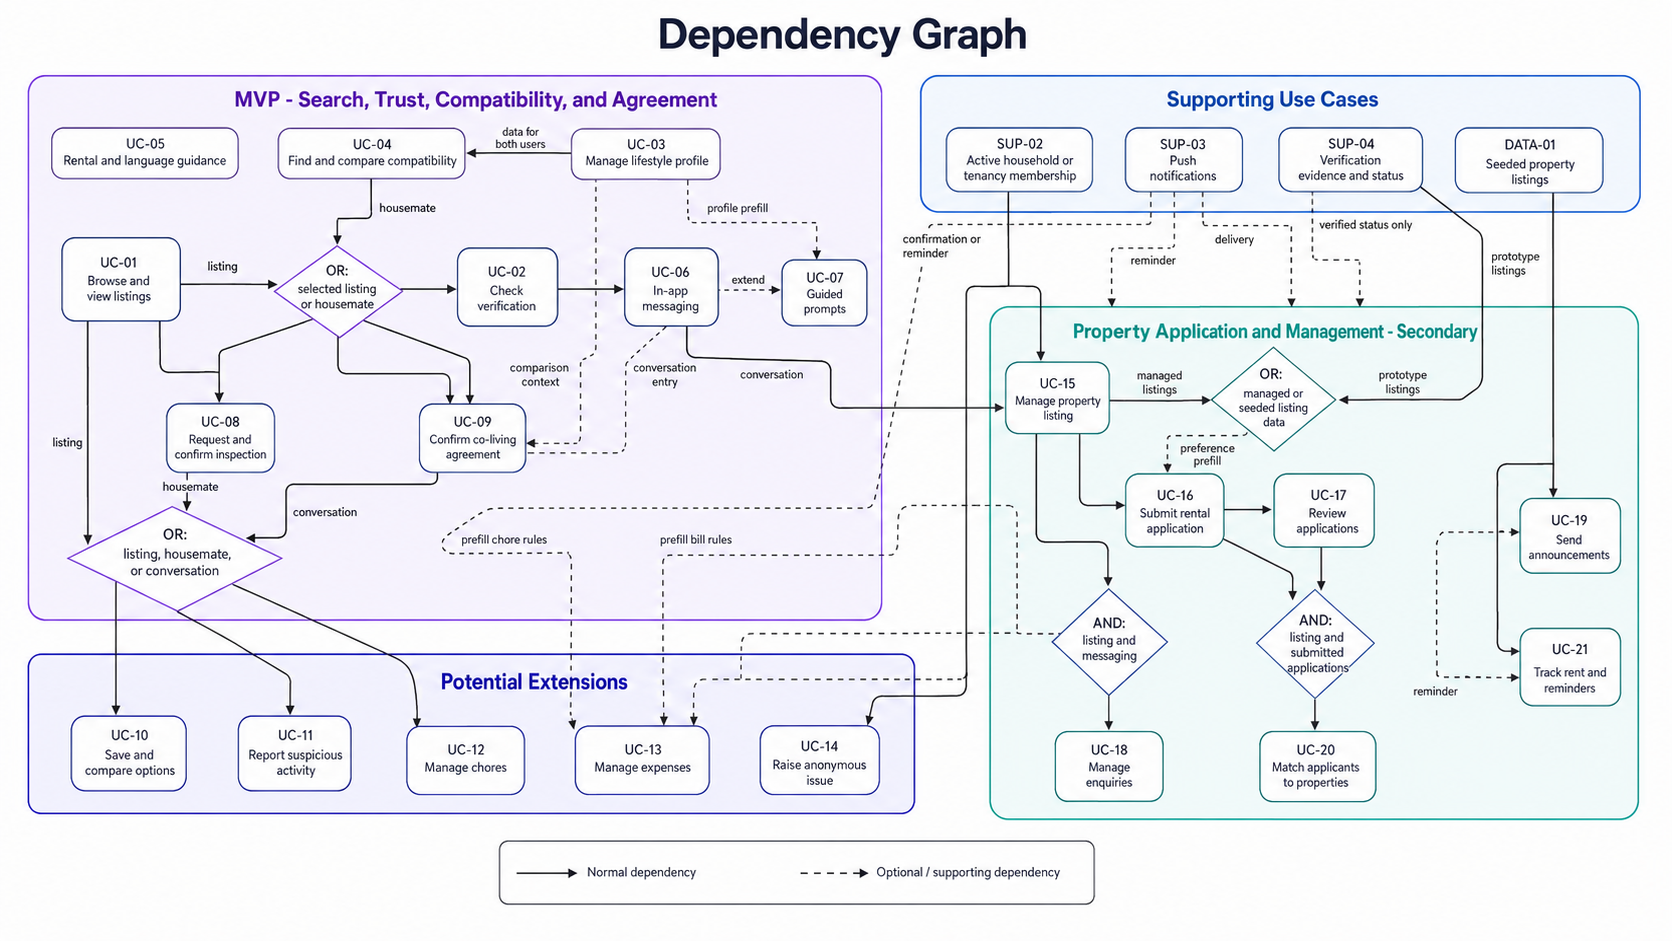
\includegraphics[width=\textwidth]{DependencyGraph.png}
    \caption{Use case dependencies for the product backlog.}
    \label{figstorydependencies}
\end{figure}

\section{First-Pass User Story Map}

\frameworknote{Required content}{Show the user activities, user tasks and release slices. Clearly identify which stories belong to Sprint 1 and which stories are scheduled for later sprints or the backlog.}

\begin{table}[H]
    \centering
    \scriptsize
    \caption{First-pass user story map template.}
    \resizebox{\textwidth}{!}{%
        \begin{tabular}{@{}L{2.6cm}L{2.8cm}L{2.8cm}L{2.8cm}L{2.8cm}L{2.8cm}@{}}
            \toprule
            Release slice & \placeholder{Activity 1} & \placeholder{Activity 2} & \placeholder{Activity 3} & \placeholder{Activity 4} & \placeholder{Activity 5}\\
            \midrule
            User task & \placeholder{Task} & \placeholder{Task} & \placeholder{Task} & \placeholder{Task} & \placeholder{Task}\\
            Sprint 1 & \placeholder{US IDs} & \placeholder{US IDs} & \placeholder{US IDs} & \placeholder{US IDs} & \placeholder{US IDs}\\
            Later sprint & \placeholder{US IDs} & \placeholder{US IDs} & \placeholder{US IDs} & \placeholder{US IDs} & \placeholder{US IDs}\\
            Backlog & \placeholder{US IDs} & \placeholder{US IDs} & \placeholder{US IDs} & \placeholder{US IDs} & \placeholder{US IDs}\\
            \bottomrule
        \end{tabular}%
    }
    \label{tabstorymap}
\end{table}

\subsection{Sprint 1 Scope and Rationale}

\frameworknote{Required content}{List the Sprint 1 stories and explain why they form a coherent, testable path through the selected concept.}

\placeholder{Insert the approved Sprint 1 story IDs and rationale.}

\section{Preliminary Prototype}

\subsection{Prototype Scope}

\frameworknote{Required content}{The preliminary prototype must correspond to the selected user stories. It must demonstrate the main Sprint 1 path and allow the related features to be tested.}

\placeholder{Describe the prototype scope, target users and main task flow.}

\subsection{Prototype Flow}

\placeholderfigure{Sprint 1 prototype flow}{5.2cm}{figprototypeflow}

\subsection{Prototype Screens}

\placeholderfigure{Preliminary prototype screens}{8.0cm}{figprototypescreens}

\section{Prototype-to-User-Story Traceability}
\label{sectraceability}

Each screen of the HTML prototype is mapped to the user story and the acceptance criteria that it demonstrates, so every Sprint~1 requirement can be traced from the backlog to an interaction that can be exercised in the prototype. Table~\ref{tabprototypetraceability} records this mapping, and the same screen identifiers are used by the test plan in Section~\ref{sectestplan}. Together the two sections close the chain that starts at a research finding and ends at a testable screen. The link column is completed once the prototype pages are hosted.

\begin{table}[H]
    \centering
    \scriptsize
    \caption{Prototype-to-user-story traceability.}
    \begin{tabularx}{\textwidth}{@{}L{1.1cm}L{2.7cm}L{1.5cm}L{2.5cm}Y L{1.5cm}@{}}
        \toprule
        Screen ID & Prototype screen & Story ID & Acceptance ID & Testable interaction & Link\\
        \midrule
        S-01 & Lifestyle profile setup & US-12 & AC-US12-04, AC-US12-05 & Complete the required preference fields, submit an incomplete form to trigger the completion prompt, save contradictory selections to trigger the conflict flag. & \\
        S-02 & Housemate and listing search results & US-13, US-11 & AC-US13-01, AC-US13-02, AC-US11-02 & Search from a university reference point, apply rent and distance filters, switch on the verified-only filter. & \\
        S-03 & Listing and profile detail & US-11, US-13 & AC-US11-03, AC-US13-03 & Open a verified and an unverified profile to compare the badge with the warning indicator, locate the affordability details. & \\
        S-04 & Compatibility comparison & US-12 & AC-US12-01, AC-US12-02, AC-US12-06 & Compare two candidate profiles through the compatibility summary, apply a strict filter to reach the zero-result broadening suggestion. & \\
        S-05 & Guided in-app chat & US-09 & AC-US09-01, AC-US09-04, AC-US09-06 & Send a first message from a guided prompt, type contact details to trigger the warning, view the unverified sender notice. & \\
        S-06 & House rule proposal & US-10 & AC-US10-01, AC-US10-04 & Propose a rule with a title, description and category, submit with missing fields to trigger the completion prompt. & \\
        S-07 & Household rules list and acknowledgement & US-10, US-02 & AC-US10-02, AC-US02-01 & Acknowledge a proposed rule as each housemate, then find the active rule in the rules list. & \\
        \bottomrule
    \end{tabularx}
    \label{tabprototypetraceability}
\end{table}

\section{Prototype Test Plan}
\label{sectestplan}

Five moderated think aloud tasks will assess the Sprint~1 path. Each task uses five participants from the target group. For each task, record whether the user finishes, how long it takes, where errors occur, and which acceptance criterion fails.

\begin{table}[H]
    \centering
    \scriptsize
    \caption{Prototype test plan.}
    \begin{tabularx}{\textwidth}{@{}L{0.8cm}L{1.8cm}L{2.2cm}Y Y L{1.4cm}@{}}
        \toprule
        Test & Stories & Participant & Task & Pass condition & Owner\\
        \midrule
        T1 & US-12 & Student new to shared housing & Complete the lifestyle profile. Try one incomplete submission and one contradictory selection. & At least 4 of 5 users finish within 3 minutes without help. The prototype identifies both invalid states. & Pranav\\
        T2 & US-11, US-13 & Student searching for a room & Find a room under \$350 per week. Identify the listing status and the profile status. Open the property details. & At least 4 of 5 users report both statuses and find the required details within 2 minutes. The unverified warning is understood. & Nicky\\
        T3 & US-12 & Student comparing housemates & Compare two profiles and choose the better match. Apply a filter that produces no result. & At least 4 of 5 users choose the higher score and state one mismatch. The broadening prompt is noticed. & Liam\\
        T4 & US-09 & International student making first contact & Contact a listing with a guided prompt. Attempt to enter personal contact details. & At least 4 of 5 users send a message within 2 minutes. A warning appears before contact details are shared. The unverified notice is understood. & Qian Cao\\
        T5 & US-02, US-10 & Student moving into a new household & Propose a quiet hours rule. Complete the acknowledgements. Find the active rule. & At least 4 of 5 users finish within 3 minutes. An incomplete proposal is rejected and the active state is clear. & Liam\\
        \bottomrule
    \end{tabularx}
    \label{tabtestoverview}
\end{table}

After each round, the team records failed criteria and revises the affected screens. The next round retests those criteria.

\section{Conclusion}

\frameworknote{Section purpose}{Summarise the selected concept, the Sprint 1 scope, the preliminary prototype and the next validation step. Do not introduce new evidence in the conclusion.}

\placeholder{Insert the conclusion after the report content is complete.}

\newpage
\section{References}

\begin{itemize}
    \item \placeholder{Insert references reused from Part 1 and any new sources used in Part 2.}
\end{itemize}

\appendix

\section{Full User Story and Use Case Mapping}
\label{appusecasemapping}

Table~\ref{tabusucmapping} links each user story to one goal level use case. The scope values match Table~\ref{tabmoscow}.

\begin{table}[H]
    \centering
    \scriptsize
    \caption{User story and use case mapping.}
    \begin{tabularx}{\textwidth}{@{}L{0.9cm}L{0.9cm}L{3.0cm}L{2.3cm}Y L{1.4cm}@{}}
        \toprule
        Story & Epic & Use case & Primary actor & Successful outcome & Scope\\
        \midrule
        US-01 & EP-02 & UC-01 Manage a chore roster & Share house resident & The user assigns rotating chores and can view completion history. & Later sprint\\
        US-02 & EP-02 & UC-02 View household rules & Share house resident & The user finds the accepted rules for the current household. & Sprint~1\\
        US-03 & EP-02 & UC-03 Propose and approve a chore system & Share house resident & The proposed system becomes active only after the required approvals. & Later sprint\\
        US-04 & EP-02 & UC-04 Log a shared expense & Share house resident & The user records the payer and the system calculates each selected share. & Later sprint\\
        US-05 & EP-02 & UC-05 Track balances & Share house resident & The user sees current balances derived from recorded expenses. & Later sprint\\
        US-06 & EP-02 & UC-06 Split a utility bill & Share house resident & The user divides a utility bill among selected household members. & Later sprint\\
        US-07 & EP-02 & UC-07 Manage household notices & Share house resident & The user posts or reads a notice within the household. & Backlog\\
        US-08 & EP-02 & UC-08 Raise an anonymous issue & Share house resident & Other residents can view the issue without seeing the reporter's identity. & Backlog\\
        US-09 & EP-01 & UC-09 Send secure messages & Accommodation seeker & The user sends and receives messages without exposing personal contact details. & Sprint~1\\
        US-10 & EP-02 & UC-10 Propose and acknowledge a house rule & Share house resident & A proposed rule becomes active after the required acknowledgements. & Sprint~1\\
        US-11 & EP-01 & UC-11 View verification status & Accommodation seeker & The user can distinguish verified and unverified profiles. & Sprint~1\\
        US-12 & EP-01 & UC-12 Compare lifestyle fit & Accommodation seeker & The user sees a compatibility result with the factors that affected it. & Sprint~1\\
        US-13 & EP-01 & UC-13 Search property listings & Accommodation seeker & The user applies location and cost filters to the available listings. & Sprint~1\\
        US-14 & EP-03 & UC-14 Receive overdue reminders & Share house resident & The user receives a reminder for an overdue chore or payment. & Later sprint\\
        US-15 & EP-03 & UC-15 Read housemate reviews & Accommodation seeker & The user reads reviews linked to confirmed former arrangements. & Backlog\\
        US-16 & EP-04 & UC-16 Track rent status & Property manager & The manager records rent status and sends an overdue reminder. & Secondary\\
        US-17 & EP-04 & UC-17 Manage property listings & Property manager & A complete listing is published and becomes searchable. & Secondary\\
        US-18 & EP-04 & UC-18 Send tenant updates & Property manager & An update reaches the current tenants of the selected property. & Secondary\\
        \bottomrule
    \end{tabularx}
    \label{tabusucmapping}
\end{table}

Supporting use cases serve several user goals. Seeded data allows the preliminary prototype to demonstrate discovery without the property manager workflow.

\begin{table}[H]
    \centering
    \small
    \caption{Supporting use cases.}
    \begin{tabularx}{\textwidth}{@{}L{1.4cm}L{4.2cm}L{3.2cm}Y@{}}
        \toprule
        ID & Supporting use case & Primary actor & Successful outcome\\
        \midrule
        SUP-01 & Manage account and role access & Registered user & The user is authenticated and receives the correct permissions.\\
        SUP-02 & Establish household or tenancy membership & Resident or property manager & Membership becomes active only after confirmation.\\
        SUP-03 & Deliver notifications & System & A reminder or update can reach a user outside the active app.\\
        SUP-04 & Manage verification evidence and status & User or system & Evidence is stored and the related status is available to the interface.\\
        \bottomrule
    \end{tabularx}
    \label{tabsupportingusecases}
\end{table}

\begin{table}[H]
    \centering
    \small
    \caption{Supporting prototype data.}
    \begin{tabularx}{\textwidth}{@{}L{1.6cm}L{3.6cm}Y@{}}
        \toprule
        Data ID & Data source & Purpose\\
        \midrule
        DATA-01 & Seeded property listings & Supplies published listings before the property manager workflow is implemented.\\
        DATA-02 & Seeded housemate profiles & Supplies completed profiles for verification and compatibility testing.\\
        \bottomrule
    \end{tabularx}
    \label{tabprototypedata}
\end{table}

\section{Prototype Screens and Links}

\frameworknote{Appendix content}{Insert full-size prototype screenshots, hosted page links and any interaction notes needed for assessment.}

\section{Jira Evidence}

\frameworknote{Appendix content}{Insert Jira backlog exports, screenshots or links showing Epics, user stories, acceptance criteria and sprint assignment.}

\end{document}
